\documentclass{article}

\usepackage[english, russian]{babel}
\usepackage[T2A]{fontenc}
\usepackage[utf8]{inputenc}

\usepackage{geometry}
\geometry{top=25mm}
\geometry{bottom=30mm}
\geometry{left=20mm}
\geometry{right=20mm}

\linespread{1}
\setlength{\parindent}{50pt}
\setlength{\parskip}{12pt}

\usepackage{graphicx}
\graphicspath{{images/}}
\usepackage{float}

\usepackage{amsmath, amsfonts, amssymb, amsthm, mathtools}
\usepackage{tikz} % графики
\usetikzlibrary{calc}
\usepackage{pgfplots} % графики

\begin{document}

\title{Линейная алгебра}
\author{}
\date{}
\maketitle

\begin{abstract}
\end{abstract}

\section{Линейное пространство} 
Линейное (векторное) пространство $\mathnormal{V}$ --- 
некоторое множество объектов произвольной природы с введенным на этом 
множестве, операциями сложения и умножения  (на число вещественное 
$\mathbb{R}$ или комплексное $\mathbb{C}$) элементов этого множества 

\begin{tikzpicture}
	% Определение координат
	\coordinate (A) at (0,0);
	\coordinate (B) at (3,2);
	\coordinate (C) at ($(A)+(B)$);
	% Рисование векторов
	\draw[->,thick] (A) -- node[below]{$\vec{a}$} (B);
	\draw[->,thick] (A) -- node[left]{$\vec{b}$} (C);
	\draw[->,thick] (A) -- node[above right]{$\vec{a}+\vec{b}$} (C);
	% Рисование координатной оси
	\draw[->] (-1,0) -- (4,0) node[right]{$x$};
	\draw[->] (0,-1) -- (0,3) node[above]{$y$};
	\end{tikzpicture}

\begin{figure}[H]
	\centering
	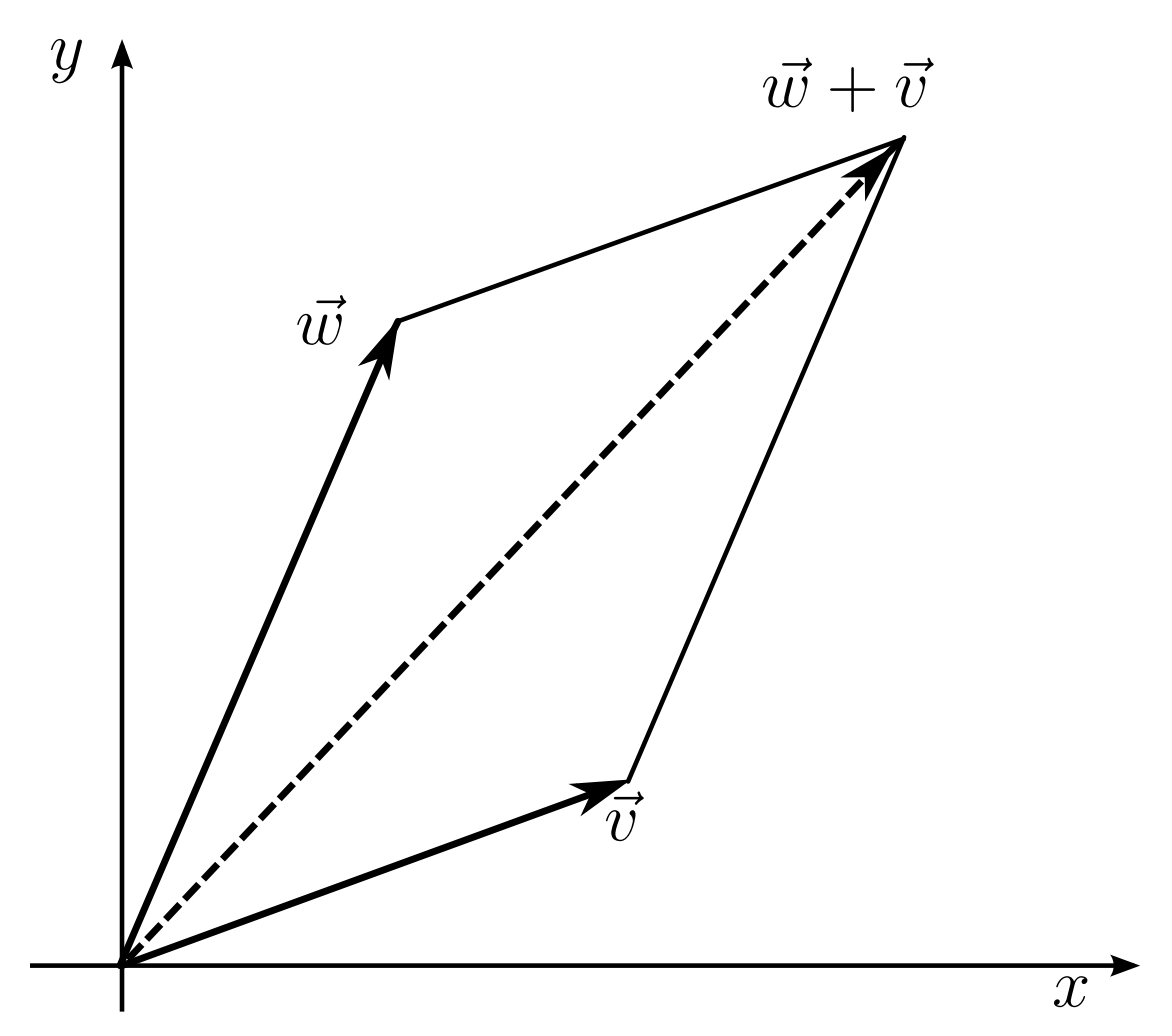
\includegraphics[width=0.75\textwidth]{1vector_sum}  
	\caption{Сумма векторов}
	% \label{fig:vector1}
\end{figure}

\begin{figure}[H]
	\centering
	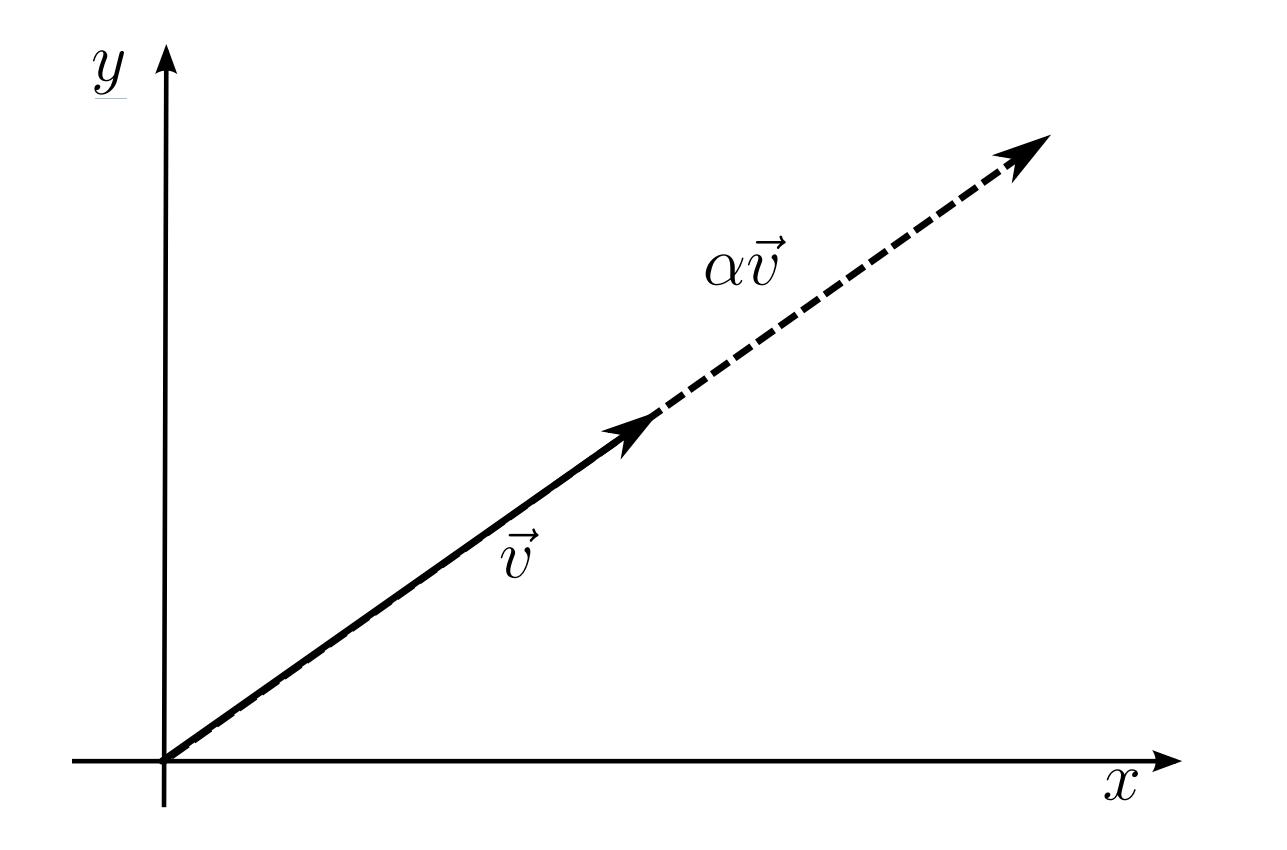
\includegraphics[width=0.75\textwidth]{2vector_proiz}  
	\caption{умножение вектора на скаляр}
	% \label{fig:vector2}
\end{figure}

Операция сложения векторов должна удовлетворять следующим четырем
аксиомам:
\begin{enumerate}
  \item коммутативность сложения: $\upsilon + \omega = \omega + \upsilon$;
  \item ассоциативность сложения: $(u + \upsilon) + \omega = u + (\upsilon + \omega)$;
	\item существование нейтрального элемента $\textbf0 \in V$, 
	такого, что $u + \textbf0 = \textbf0+u = u$ для любого вектора u;
	\[\exists0;\quad u+0=0+u=u\]
	\item существование для любого $u \in V$ обратного элемента $u^{-1}$, 
	такого, что $u+u^-1 = u^-1+u = 0$.
	\[\forall u \in \mathnormal{V} \quad \exists u^-1 ; u + u^-1 = 0  \]
\end{enumerate}

Операция умножения вектора на скаляр (например, на вещественное число) должна подчиняться таким четырем аксиомам:
\begin{enumerate}
  \item умножение любого вектора $\upsilon$ на $1 \in \mathbb{R}$ должно давать тот же самый вектор $\upsilon$;
  \item ассоциативность операции умножения: $\alpha(\beta \cdot \upsilon) = (\alpha \cdot \beta) \upsilon$;
	\item дистрибутивность относительно сложения векторов: $\alpha(\upsilon + w) = \alpha \upsilon + \alpha w$;
	\item дистрибутивность относительно сложения скаляров: $(\alpha + \beta)\upsilon = \alpha\upsilon + \beta\upsilon$.
\end{enumerate}

\subsection{фыва}
asdf
\end{document}
